\documentclass[12pt]{report}

\usepackage{url}
\usepackage{xspace}
\usepackage{fancybox}
\usepackage{cuthesis}
\usepackage{graphicx}
\usepackage{booktabs}
\usepackage{makecell}
\usepackage{csquotes}
\usepackage{multirow}
\usepackage{pdflscape}
\usepackage{subfigure}

%\usepackage{graphicx}
%\usepackage{balance}
\usepackage{amssymb,amsmath}
%\usepackage{wrapfig}
%\usepackage{multirow}
\usepackage{graphicx}
\usepackage{algorithm}
\usepackage{algorithmic}
%\usepackage{times}
%\usepackage{cite}
%\usepackage{fancybox}
%\usepackage{color}
%\usepackage{array}
%\usepackage{subfigure}
%\usepackage{epstopdf}
%\usepackage{booktabs}
%\usepackage{caption,fixltx2e}
\usepackage[flushleft]{threeparttable}
%\usepackage{subfig}
%\usepackage{xspace}
%\usepackage[hyphens]{url}
%\usepackage[hidelinks]{hyperref}
%\hypersetup{breaklinks=true}
%\urlstyle{same}
%\def\UrlBreaks{\do\/\do-} %to break the urls, all in one line
%\newcommand{\ian}[1]{\textcolor{blue}{{\it [Ian: #1]}}}
%\newcommand{\emad}[1]{\textcolor{green}{{\it [Emad: #1]}}}
%\newcommand{\todo}[1]{\textcolor{red}{{\it [TODO: #1]}}}



\linespread{1.6}

\author{Muhammad Moiz Arif}
\title {Thesis Title Here}
\degree{Master of Applied Science in Software Engineering}
\dept  {Computer Science and Software Engineering}

%%%%%%%%%%%%%%%%%%%%%%%%%%%%%%%%%%%%%%%%%%%%%%%%%%%%%%%%%
% define commands for frequently used words or phrases
%%%%%%%%%%%%%%%%%%%%%%%%%%%%%%%%%%%%%%%%%%%%%%%%%%%%%%%%%
% \newcommand{\SATD}{self-admitted technical debt\xspace}

%%%%%%%%%%%%%%%%%%%%%%%%%%%%%%%%%%%%%%%%%%%%%%%%%%%%%%%%%
% define commands for your RQs
%%%%%%%%%%%%%%%%%%%%%%%%%%%%%%%%%%%%%%%%%%%%%%%%%%%%%%%%%
\newcommand{\chapterIIIrqi}{\textbf{RQ:}}
\newcommand{\chapterIVrqi}{\textbf{RQ1. \\}}
\newcommand{\chapterIVrqii}{\textbf{RQ2. \\}}
\newcommand{\chapterIVrqiii}{\textbf{RQ3. \\}}


%%%%%%%%%%%%%%%%%%%%%%%%%%%%%%%%%%%%%%%%%%%%%%%%%%%%%%%%
% define command to create a conclusion box to answer your RQs
%%%%%%%%%%%%%%%%%%%%%%%%%%%%%%%%%%%%%%%%%%%%%%%%%%%%%%%%
\newcommand{\conclusionbox}[1]{%
    \vspace{6mm}
    \framebox[0.95\textwidth][c]{%
        \parbox[b]{0.92\textwidth}{%
            {\it #1}
        }
    }
    \vspace{6mm}
}


\begin{document}

\begin{abstract}

Large software systems often undergo performance tests to ensure their capability to handle expected loads. These performance tests often consume large amounts of computing resources and time since heavy loads need to be generated. Making it worse, the ever evolving field requires frequent updates to the performance testing environment. In practice, virtual machines (VMs) are widely exploited to provide flexible and less costly environments for performance tests. However, the use of VMs may introduce extra overhead (e.g., a higher than expected memory utilization) to the testing environment and lead to unrealistic performance testing results. Yet, little or no research has studied the overhead and impact on test results of using VMs in performance testing activities. 

To evaluate the discrepancy between the performance testing results from virtual and physical environments, we perform a case study on two open source systems - namely Dell DVD Store and CloudStore. We conduct the same performance tests in both virtual and physical environments and compare the performance testing results based on the three aspects that are typically examined for performance testing results: 1) individual performance metrics (e.g. CPU Time from virtual environment vs. CPU Time from physical environment), 2) the relationship among performance metrics (e.g. correlation between CPU and I/O) and 3) performance models that are built to predict system performance. Our results show that 1) individual performance metrics from virtual and physical environments do not follow the same distribution hence practitioners cannot simply use a scaling factor to compare the performance between environments,  2) correlations among performance metrics in virtual environments are different from those in physical environments 3) statistical models built based on the performance counters from virtual environments are different from the models built from physical environments suggesting that practitioners cannot use the performance testing results across virtual and physical environments. In order to assist the practitioners leverage performance testing results in both environments, we also investigate ways to transform results from virtual and physical environments and performance metrics based on deviance may reduced the discrepancy between performance metrics. Overall, we recommend that practitioners should not simply assume that performance testing results done on virtual environments will be the same in physical environments.

\end{abstract}

\begin{acknowledgments}

Thesis acknowledgments.

\end{acknowledgments}

\begin{publications}

The following publications are related to this thesis:

\begin{enumerate}

\item \textbf{Moiz} 

%\item \textbf{Moiz}, 
\end{enumerate}

\end{publications}

\chapter{Introduction}
\label{introduction}
% -*- root: cuthesis_masters.tex -*-  

%At the core of any software system is the software team who develop it...

\section{Introduction}
%Cloud computing has eliminated the need for hardware decisions. It is now a significant part of the IT industry incorporating not only the leading names like \textit{Facebook, Amazon, Google} etc but also small-scaled business ventures that are migrating on to a cloud based environment. According to a survey \textit{'survey'}, up to 70\% of the companies are moving from conventional physical data servers? to cloud based servers. The primary concerns when migrating are, usually, costs, availability performance etc of the system. 
%Software Performance Engineering(SPE) incorporates all the software engineering activities carried out during the project's lifecycle required to meet the software's performance requirements.
%These performance requirements ensure that the user requests are served are in a timely manner and the software's response time does not degrade with the increase in workload i.e. users. In the midst of todays large-scale software systems, (e.g.Amazon and Google's Gmail), SPE plays a vital role as most of the failures are associated with performance than with feature bugs. A second's downtime of amazon.com would cost millions of dollars. One of the recent examples in this regard was the roll-out failure of healthcare.gov. Another example was the crash of Facebook which caused NASDAQ a high monetary misfortune. 
%To avoid performance failures, software performance engineers use performance testing. The tests are used to exercise the subject system which is under test. To exercise this system, it is subjected to different workloads. These tests are designed to uncover performance bottlenecks or a test objective like maximum operational capacity. 
%The goal of performance testing is to test how the system responds are realistic workloads. Therefore performance test are composted of test workload and configuration of SUT which represents a field like environment. 
%The goal of this study is to compare the performance of a SUT in heterogeneous environments. Due to lack of resources and constant requirement of evolution of the testing environment practitioners often rely on testing done in virtual environments. However, the road that leads to the reliability of performance activities done in virtual environments still remains undiscovered. 
%Performance is a big deal
Software performance assurance activities play a vital role in the development of large software systems. These activities ensure that the software meets the desired performance requirements~\cite{futureofspe}. Often however, failures in large software systems are due to performance issues rather than functional bugs~\cite{tailatscale, foo2010mining}. Such failures lead to the eventual decline in quality of the system with reputational and monetary consequences~\cite{costofdowntime}. For instance, Amazon estimates that a one-second page-load slowdown can cost up to \$1.6 billion~\cite{amazononesec}. 

%The impact from performance issues on system reliability would also lead to serious reputational issues.

%an interruption in the Amazon Web Service lead to the disruption of Quora, Reddit, Foursquare and numerous other web sites~\cite{amazondown}. 

%In the software ecosystem, performance assurance activities play a vital role \cite{Shang:2015:ADP:2668930.2688052}. In essence, these activities ensure a consistent software functionality. The trend of dedicating a large chunk of costs, in some cases even exceeding the cost of development \cite{bertolino2007software} to such performance assurance activities is now not unusual. In fact, most of the problems in the field are due to performance related issues \cite{foo2010mining} . A failure here would not only include an eventual decline in the quality of the software but also monetary and temporal losses. That is why companies like \textit{Facebook, Amazon and Google} are committed to achieve excellence in this regard. \cite{jackson2010performance}

% Practitioners use performance tests
In order to mitigate performance issues and ensure software reliability, practitioners often conduct performance tests~\cite{futureofspe}. Performance tests apply a workload (e.g., mimicking users' behavior in the field) on the software system~\cite{ranjanbook,Syer2016}, and monitor performance metrics, such as CPU usage, that are generated based on the tests. Practitioners use such metrics to gauge the performance of the software system and identify potential performance issues (such as memory leaks~\cite{markicsm2013} and throughput bottlenecks~\cite{5635038}).

%Performance tests are subjected to highlight system's performance which are congruent to a field-like load~\cite{Shang:2015:ADP:2668930.2688052, Syer2016}. For example, to investigate the performance bottlenecks, the maximum throughput of the system~\cite{syer2014maintenance} or other the non-functional performance requirements.

%The objective behind performance regression testing is to identify if there exists a lapse in performance for the newer version of the software compared to the previous versions. The system is tested by applying a fixed load which is congruent to a field-like load \cite{Shang:2015:ADP:2668930.2688052} \cite{foo2010mining} \cite{5306331}. The performance analysts then look for deviations between metrics values compared to the earlier versions. Examples of factors causing performance lapse may be because of high CPU utilization or a memory leak. \cite{5306331}. As there are no benchmarks for measuring the software performance cross environments, and with little or no time dedicated to performance assurance activities practitioners often find it hard to test and analyze the results of regression testing.

%The need for performance testing environments to advance and evolve is continually augmenting and so is the cost associated with the environment~\cite{stpmag, bertolino2007software}. 

%One of challenges practitioners face is the lack of available resources for performance testing. For instance

%People perform things on virtual environments
Since performance tests are often performed on large-scale software systems, the performance tests often require many resources~\cite{ranjanbook}. Moreover, performance tests often need to run for a long period of time in order to build statistical confidence on the results~\cite{ranjanbook}. In addition, such testing environment needs to be easily configurable such that a specific environment can be mimicked, reducing false performance issues. For example, issues that are related to the environment. Therefore, to address such challenges, virtual environments (i.e., VMs) are often leveraged for performance testing~\cite{whyvirtualisbetter, vmwarehighcost, whyvirtualisbetter}. The flexibility of virtual environments enables practitioners to easily prepare, customize, use and update performance testing environments in an efficient manner.

%Making it worse, the diversified and ever-changing users' behaviour forces the testing environments to be frequently customized and updated~\cite{Syer2016}.

%More importantly, performance testing is often last stage of the software development lifecycle which forces the managers to dedicate a minimal time for performance testing which can even span out to days. That's why practitioners prefer testing the system in a virtual environment~\cite{whyvirtualisbetter, vmwarehighcost}. The choice of running the performance assurance activities in a virtual environment is also based on the complexity of the large scale software systems. This enforces a virtual set up of the environment which saves resources and is easier to set up according to the desired needs~\cite{VMWarePowerCLIBlog, seetharaman2006test}. 

% No one looked at the applicability across platforms
%However, a major question that lingers is that \textbf{are performance tests executed in a virtual environment representative of what happens in the physical environment?}. This question is particularly important since 1) virtual environments are highly leveraged in practice~\cite{Nguyen:2012:ADP:2188286.2188344,xiong2013vperfguard} and 2) prior work has shown that using virtual machines imposes a hidden overhead that is rarely considered~\cite{menon2005diagnosing}, impacting the reliability of performance test results performed in virtual environments. 

Prior studies show that virtual environments are widely exploited in practice~\cite{Cito:2015:MCA:2786805.2786826,Nguyen:2012:ADP:2188286.2188344,xiong2013vperfguard}. Studies have investigated the overhead that is associated with virtual environments~\cite{menon2005diagnosing}. Such overheads may not impose effect on the results of performance tests carried out in physical and virtual environments. For example, if the performance (e.g., throughput) of the system follows the same trend (or distribution) in physical and virtual environments, such overhead would not significantly impact on the practitioners who examine the performance testing results. To the best of our knowledge, the discrepancy between performance testing results in virtual and physical environments has never been studied. Exploring, identifying and minimizing such discrepancy will help practitioners and researchers understand and leverage performance testing results from virtual and physical environments. Without knowing if there exists a discrepancy between the performance testing results from the two environments practitioners cannot rely on the performance assurance activities carried out in the virtual environment or vice versa. Once the discrepancy is identified, the performance results could be evaluated more accurately.



%Whether virtual environments are applicable in performance assurance activities or if they can be relied to behave equivalent to the physical servers still remains questionable. There have been limited instances of diagnosis of performance overheads~\cite{menon2005diagnosing} in the domain of performance testing however no concrete conclusions have been drawn yet. 

%The goal of our study is evaluating the discrepancy between the performance testing results from virtual and physical environments. 
%Additionally, we investigated if the performane tests done in virtual environments are repeatable or not. 
%Additionally, if they do not belong to the same population, then how impactful and effective are the prevalent discrepancies for a model-based regression testing approach.    


%what we do
In this thesis, we perform a study on two open-source systems, DS2~\cite{delldvd} and CloudStore~\cite{cloudstore}, where performance tests are conducted on virtual and physical environments. Our study focuses on the discrepancy between the two environments, the impact of discrepancy on performance testing results and highlights potential opportunities to minimize the discrepancy. In particular, we compare performance testing results from virtual and physical environments based on the three widely examined aspects, i.e., individual performance metric, the relationship between the performance metrics and models that predict performance. 
%by running performance tests in both virtual and physical environments. We compare the performance test results that are generated from both the environments. In particular, we compare the performance testing results by 1) examining individual performance metric, 2) examining relationship among performance metrics and 3) building statistical models using performance metrics. 

%what we find


%Our findings highlight the need of awareness of the discrepancy between performance testing results in virtual and physical environments, and the need to research efforts on investigating how to improve the use of both virtual and physical environments to ensure system reliability.

%We leverage a heatmap to visualize the changes in correlations among performance metrics and the system load metric.

% cannot apply on the performance metrics collected from another environments (with high prediction error), even after normalizing the performance metrics.


%In particular, we first compare the performance metrics values and distributions. We then investigate the correlation of performance counters to the generated load. Finally, we build statistical models to help us reach conclusions. 
%We observed that majority of the performance counters do not belong to the same family of distribution. We also observed that the metric that are highly correlated with the load are not the same across both our subject systems.
%We concluded that due to the discrepancies present in the virtual environment, we can not rely on performance evaluated in the virtual environment as is. We then apply scaling techniques to the metrics generated in the virtual environment to build linear regression models. We concluded that the performance metrics in the virtual environment are not identical copies of the metrics in the physical environment. 


% to determine and compare the distributions. This is achieved by comparing plots and finding correlation between the metrics cross-environments. We use generalized linear regression models, as used in the performance assurance activities \cite{Shang:2015:ADP:2668930.2688052}, to determine the extent of the comparison between metrics. If the metrics are transferable between the environments, we should expect to see a low percentage error. We chose to build our regression models based on multiple performance metrics to see the effect of the clustered performance metrics. 

%We diffuse our findings by answering the following research questions:

%\begin{description}
%	\item[$\bullet$] RQ1: Do performance metrics from physical and virtual environments belong to the same population?
%	\item[$\bullet$] RQ2: Is the metric correlation with load same cross-environments?
%	\item[$\bullet$] RQ3: Do performance metrics from different environments impact performance modeling?

%\end{description}

\section{Research Hypothesis}
Prior research and our industrial experience lead us to an investigation based on the following hypothesis:
%	\fbox{%
%		\parbox{\textwidth}{%
%			\textit{
%			For large-scale software systems, performance assurance activities are carried primarily in virtual environments. There is little research regarding the reliability of testing in a different environment compared to physical. We hypothesize that for software testing activities there exists a discrepancy between physical and virtual environments. We believe that the approaches used so far do not scale well. 
%			Furthermore, we believe practitioners should be aware of such existing discrepancies when analyzing software performance in a foreign environment.
%				   }
%		}%
%	}
	
\begin{framed}
		\textit{For large-scale software systems, performance assurance activities are carried primarily in virtual environments. There is little research regarding the reliability of testing in a different environment compared to physical. We hypothesize that for software testing activities there exists a discrepancy between physical and virtual environments. We believe that the approaches used so far do not scale well.} 
		\par 	
		\textit{Furthermore, we believe practitioners should be aware of such existing discrepancies when analyzing software performance in a foreign environment.}
\end{framed}



\section{Thesis Overview}

%The rest of the paper is organized as follows. Section~\ref{sec:related} presents the background and related work. Section~\ref{sec:case} presents the case study setup. Section~\ref{sec:results} presents the results of our cases study, followed by a discussion of our results in Section~\ref{sec:discussion}. Section~\ref{sec:threats} discusses the threats to validity of our findings. Finally, Section~\ref{sec:conclusion} concludes this paper.

\textbf{Chapter 2: Literature Review:} In this chapter, we discuss the related work that has discussed performance assurance activities carried out in virtual environments and the associated overhead caused by it. The chapter is divided in two parts:

	\textbf{Part I:} Addresses the methodologies that are used to detect performance anomalies. We present the work sub divided into three categories: individual performance metrics, relationship among performance metrics, statistical modeling based on performance metrics.   
	
    \textbf{Part II:} Addresses the work that points to the overheads present in virtual environments. We present the state-of-the-art approaches used to detect performance anomalies and how such approaches helps us in detection of overheads. The chapter wraps up by comparing the current limitations and our work in the field of performance engineering.

From the literature review, we deduced that a lot of work has been affiliated to the generation of performance alarms and the detection of performance issues however little work has highlighted the reliability of testing done in virtual environments.
\\

\noindent\textbf{Chapter 3: Testing For the Ubiety of Discrepancy:} In this chapter, we perform case studies on two open source subject systems. We generate the performance metrics by applying realistic and varying workloads in identically set up physical and virtual environments. Followed up data cleansing and removing any reasonable outliers present in our data. Next, we analyze the performance metrics in three possible ways: individually, as a collection, and as an input to statistical models. 
\\

\noindent\textbf{Chapter 4: Studying the impact of modifying the virtual environment}
Furthermore, we elaborate and solidify the conclusion drawn by discussing possibilities as how the use of virtual environments may effect our results: by changing the type of the virtual machine, by modifying the allocated resources and testing the repeatability(hence the stability) of our chosen virtual environment.
Lastly, we discuss the threats to validity for this thesis.
\\


\section{Thesis Contributions}

The major contributions of thesis are as follows:

\begin{itemize}
	\item An extensive review of the state of the art in software performance activities carried out in virtual environments. Such a review is necessary for the practitioners to be aware of the hiccups associated to software performance in virtual environments.
	
	\item We conclude performance metrics have different shapes of distributions and trends in virtual environments compared to physical environments. There are large differences in correlations among performance metrics measured in virtual and physical environments.
	\item We highlight statistical models using performance metrics from virtual environments do not apply to physical environments (i.e., produce high prediction error) and vice versa.
	\item  We examined the feasibility of using normalizations to help alleviate the discrepancy between performance metrics. We find that in some cases, normalizing performance metrics based on deviance may reduce the prediction error when using performance metrics collected from one environment and applying it on another. 
	\item We demonstrate that practitioners cannot assume that their performance tests that are observed on one environment will necessarily apply to another environment. The overhead from virtual environments does not only impact the scale of the performance metrics, but also impacts the relationship among performance metrics. On the other hand, we find that practitioners who leverage both, virtual and physical environments, may be able to reduce the discrepancy that may arise due to the environment (i.e., virtual vs. physical) by applying normalization techniques.
\end{itemize}

\chapter{Literature Review}
\label{literature_review}
% -*- root: cuthesis_masters.tex -*-

In this chapter we present related work on ...


\chapter{Chapter 3 Title}
\label{chapter3}
% -*- root: cuthesis_masters.tex -*-



\begin{landscape}

\begin{figure}[thb]
	%\centering
	%\vfil
	\vspace*{15ex}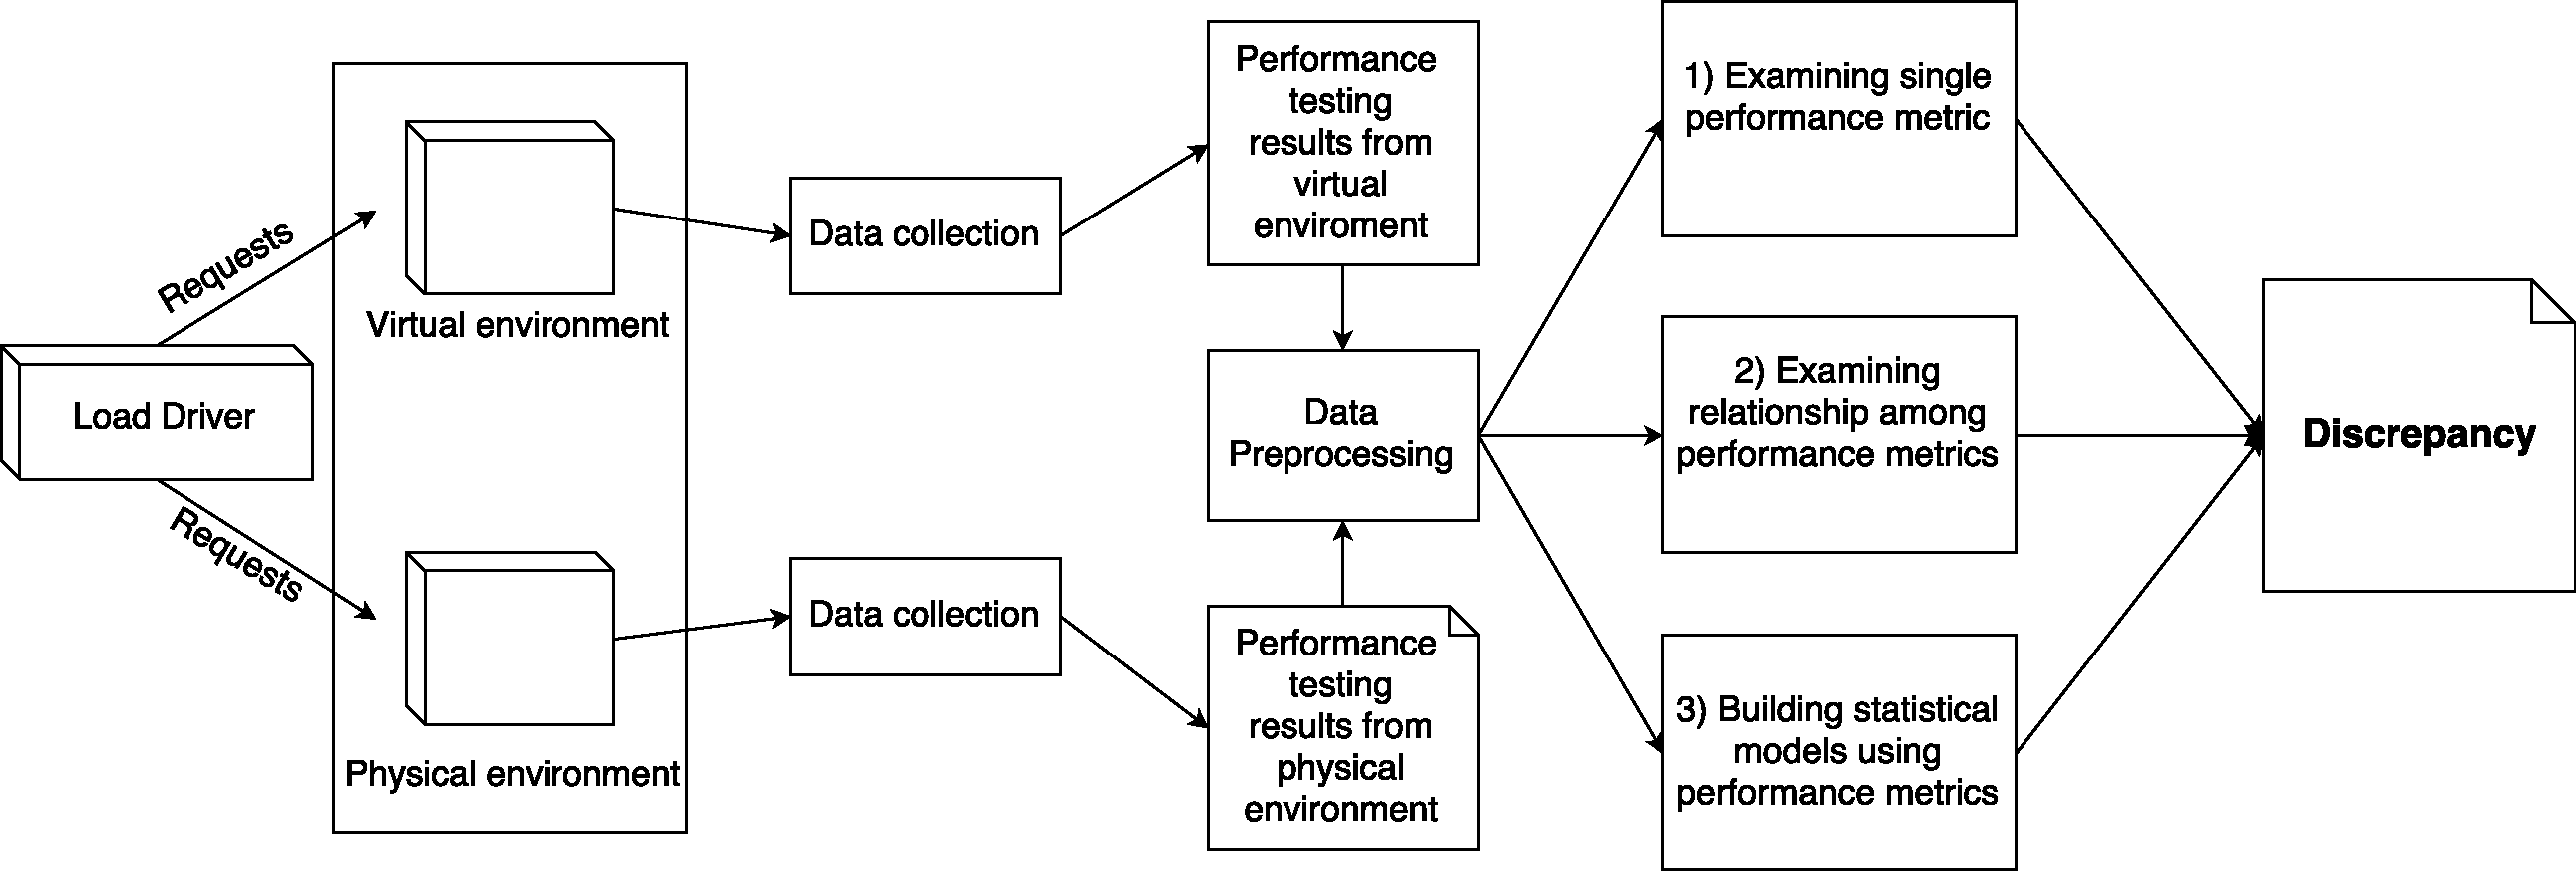
\includegraphics[width=1.5\textwidth]{figures/overview_ls}
	\caption{Overview of our case study setup.}
	%\captionsetup{justification=centering}
	\label{fig:Approach}
\end{figure}

\end{landscape}

\section{Approach}
\label{chap3:sec:approach}


The goal of our case study is to evaluate the discrepancy between performance testing results from virtual and physical environments. We deploy our subject systems in two identical environments (physical and virtual) with the same hardware. A load driver is used to exercise our subject systems. After the collection and processing of the performance metrics we analyze and draw conclusions based on: 1) single performance metric 2) relationship between performance metrics and 3) statistical models based on the performance metrics. An overview of our case study setup is shown in Figure~\ref{fig:Approach}.


\subsection{Subject Systems}
Dell DVD Store (DS2)~\cite{delldvd} is an online multi-tier e-commerce web application that is widely used in performance testing and prior performance engineering research~\cite{Shang:2015:ADP:2668930.2688052,Nguyen:2012:ADP:2188286.2188344, jackicsm2009}. We deploy DS2 (SLOC $>$ 3,200) on an Apache (Version 3.0.0) web application server with MySQL 5.6 database server~\cite{mysql}. CloudStore~\cite{cloudstore}, our second subject system, is an open source application based on the TPC-W benchmark~\cite{tpcw}. CloudStore (SLOC $>$ 7,600) is widely used to evaluate the performance of cloud computing infrastructure when hosting web-based software systems and is leveraged in prior research~\cite{tarekmsr16}. We deploy CloudStore on \textit{Apache Tomcat}~\cite{tomcat} (version 7.0.65) with MySQL 5.6 database server~\cite{mysql}.


\subsection{Environmental Setup}

The performance tests of the two subject systems are conducted on three machines in a lab environment. Each machine has an Intel i5 4690 Haswell Quad-Core 3.50 GHz CPU, with 8 GB of memory, 100GB SATA storage and connected to a local gigabyte ethernet. The first machine hosts the application servers (Apache and Tomcat). The second machine hosts the MySQL 5.6 database server. The load drivers were deployed on the third machine. We separate the load driver, the web/application server and the database server on different machines in order to mimic the real world scenario and avoid interference among these processes. For example, isolating the application and database driver would ensure that the processor is not overused. The operating systems on the three machines are Windows 7. We disable all other processes and unrelated system services to minimize their performance impact. Since our goal is to compare performance metrics in virtual and physical environments, we setup the two different environments, as follows:
\\

\noindent \textbf{Virtual environment.} We install one Virtual Box (version 5.0.16) and create only one virtual machine on one physical machine to avoid any interference between virtual machines. For each virtual machine, we allocate two cores and three gigabytes of memory, which is well below capacity to make sure we are not topping out and pushing our configuration for unrealistic results. Virtual machines typically have an option of using disk pass-through\cite{whatisdiskpassthrough}. However, disk pass-through prevents the quick deployment of an existing virtual machine image that's designed for performance testing and quick execution of performance tests~\cite{diskpassthrough}. Hence, we opt to disable disk pass-through since it is unlikely to be used in practice. The network of the virtual machine is set up based on network address translation (NAT) configuration\cite{NAT_config}. The network traffic of the workload was generated on a dedicated load machine to keep our experiments as close to the real-world as possible.
\\


\noindent \textbf{Physical environment.} We used the same hardware as the virtual environment to set up our physical environments. To make the physical environment similar to the virtual environment, we only enable two cores and three gigabytes of memory for each machine for the physical environment. 

\subsection{Performance tests}

DS2 is released with a dedicated load driver program that is designed to exercise DS2 for performance testing. We used the load driver to conduct performance testing on DS2. We used Apache JMeter~\cite{apachejmeter} to generate a workload to conduct the performance tests on CloudStore. For both subject systems, the workload of the performance tests is varied randomly and periodically in order to avoid bias from a consistent workload. The variation was identical across environments. The workload variation was introduced by the number of threads. A higher number of threads represents a higher number of users accessing the system. Each performance test is run after a 15 minute warming up period of the system and lasts for 9 hours. We chose to run the test 9 hours ensuring that our sample sizes have enough data points for our results to be statistically significant.
The nature of our performance tests was based on our related studies mentioned in section 2.2. To ensure the consistency between the performance tests, we restored the environments followed by a restart of the systems after every test.


\subsection{Data collection and preprocessing}

\noindent \textbf{Performance metrics.} We used \textit{PerfMon}~\cite{perfmon} to record the values of performance metrics. \textit{PerfMon} is a performance monitoring tool used to observe and record performance metrics such as CPU utilization, memory usage and disk IOs. We run \textit{PerfMon} on each of the application server and database server machines. We record all the available performance metrics that can be monitored on a single process by \emph{PerfMon}. In order to minimize the influence of \textit{Perfmon}, we monitor only the performance of the two processes of the application server and database server on the two dedicated machines. We recorded the performance metrics with an interval of 10 seconds. In total, we recorded 44 performance metrics.
\\

\noindent \textbf{System throughput.} We used the application server's access logs from Apache and Tomcat to calculate the throughput of the system by measuring the number of requests per minute. The two datasets were then concatenated and mapped against requests using their respective timestamps.

Since an end user will consider a system as a whole, we combine the performance datasets from our application and database servers. In order to combine the two datasets of performance metrics and system throughput, and to minimize noise of the performance metric recording, we calculate the mean values of the performance metrics every minute. Then, we combine the datasets of performance metrics and system throughput based on the time stamp on a per minute basis. A similar approach has been applied to address mining performance metrics challenges~\cite{foo2010mining}.

The goal of our study is to evaluate the discrepancy between performance testing results from virtual and physical environments, particularly considering the impact of discrepancy on the analysis of such results. Our experiments are set in the context of analyzing performance testing data, based on the related work. Shown in Section~\ref{sec:related}, prior research and practitioners examine performance testing results in three types of approaches: 1) examining a single performance metric, 2) examining the relationship between performance metrics and 3) building statistical models using performance metrics. Therefore, our experiments are designed to answer three research questions, where each questions corresponds to one of the types of analysis above.



\subsection{Are the trend and distribution of a single performance metric similar across environments?}
\label{sec:individual}

\noindent \textbf{Motivation.}
The most intuitive approach of examining performance testing results is to examine every single performance metric. As shown in Section~\ref{sec:relatedindividual}, prior studies propose different approaches that typically compare the distribution or trend of each performance metric from different tests. Due to influences from testing environments, performance testing results are not expected to be identical in raw values. However, the shape of the distribution and the trend of the metrics should be similar. For example, if in one environment, we observe that Memory has an increasing trend while the increasing trend is not seen in another environment, we observe a discrepancy. In addition, the distribution differences between two test results should not be statistically significant. Therefore, we use quantile-quantile (Q-Q) plot and normalized Kolmogorov-Smirnov (KS) tests to examine the differences in trends and shape of the distributions. 
\\

\noindent \textbf{Approach.} 
After running and collecting the performance metrics, we compare every single performance metric between the virtual and physical environments. Since the performance tests are conducted in different environments, intuitively the scales of performance metrics are not the same. For example, the virtual environment may have higher CPU usage than the physical environment. Therefore, instead of comparing the values of each performance metric in both environments, we study whether the performance metric follows the same shape of the distribution and the same trend in virtual and physical environments. 

First, we plot a quantile-quantile (Q-Q) plot~\cite{qqplots} for every performance metric in two environments. A Q-Q plot is a plot of the quantiles of the first data set against the quantiles of the second data set. We also plot a 45-degree reference line on the Q-Q plots. If the performance metrics in both environments follow the same shape of the distribution, the points on the Q-Q plots should fall approximately along this reference (i.e., 45-degree) line. A large departure from the reference line indicates that the performance metrics in the virtual and physical environments come from populations with different shapes of distributions, which can lead to a different set of conclusions. For example, the virtual environment has a CPU's utilization spike at a certain time, but the spike is absent in the physical environment. 

Second, to quantitatively measure the discrepancy, we perform a Kolmogorov-Smirnov test~\cite{kstest} between every performance metric in the virtual and physical environments. Since the scales of each performance metric in both environments are not the same, we first normalize the metrics based on their median values and their median absolute deviation: 
\begin{equation}
\label{equ:mad}
M_{normalized}=\frac{M-\tilde{M}}{MAD(M))}		
\end{equation}

where $M_{normalized}$ is the normalized value of the metric, $M$ is the original value of the metric, $\tilde{M}$ is the median value of the metric and $MAD(M)$ is the median absolute deviation of the metric~\cite{walker1929studies}. The Kolmogorov-Smirnov test gives a p-value as the test outcome. A p-value $\leq$ 0.05 means that the result is statistically significant, and we may reject the null hypothesis (i.e., two populations are from the same distribution). By rejecting the null hypothesis, we can accept the alternative hypothesis, which tells us the performance metrics in virtual and physical environments do not have the same distribution. We choose to use the Kolmogorov-Smirnov test since it does not have any assumption on the distribution of the metrics.

Finally, we calculate Spearman's rank correlation between every performance metric in the virtual environment and the corresponding performance metric in the physical environment, in order to assess whether the same performance metrics in two environments follow the same trend during the test. Intuitively, two sets of performance testing results without discrepancy should show a similar trend, i.e., when memory keeps increasing in the physical environment (like memory leak), the memory should also increase in the virtual environment. We choose Spearman's rank correlation since it does not have any assumption on the distribution of the metrics. 
\\

\noindent \textbf{Results.}
\noindent \textbf{Most performance metrics do not follow the same shape of the distribution in virtual and physical environments.} Figure~\ref{fig:qqds2} and \ref{fig:qqcs} show the Q-Q plots by comparing the quantiles of performance metrics from virtual and physical environments. We only present Q-Q plots for CPU user time, IO data operations/sec and memory working set for both application sever and database server. For complete results please refer Chapter \ref{appendix}.



\begin{figure}[tp]]
	\centering
	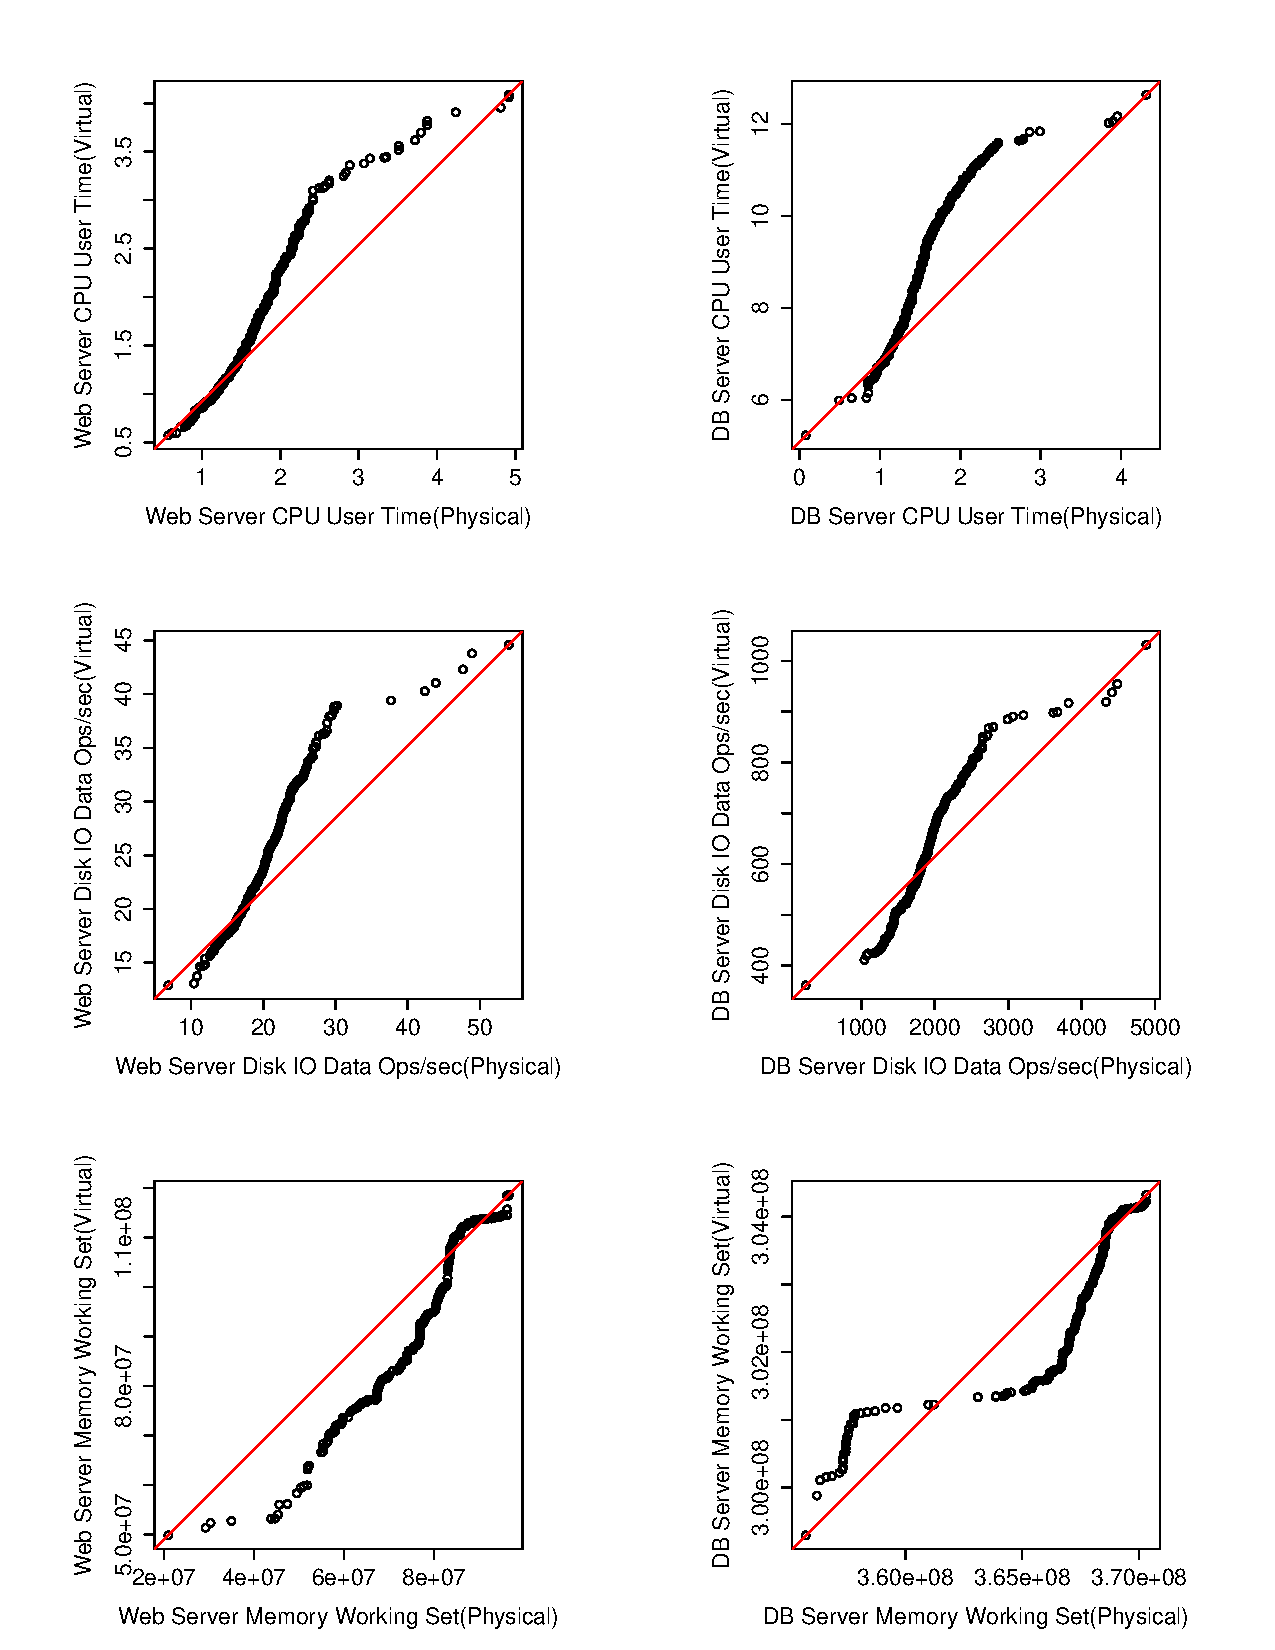
\includegraphics[width=0.9\columnwidth]{figures/DS2_qq.pdf}
	\caption{Q-Q plots for DS2.}
	\label{fig:qqds2}
\end{figure}



\begin{figure}[tp]
	\centering
	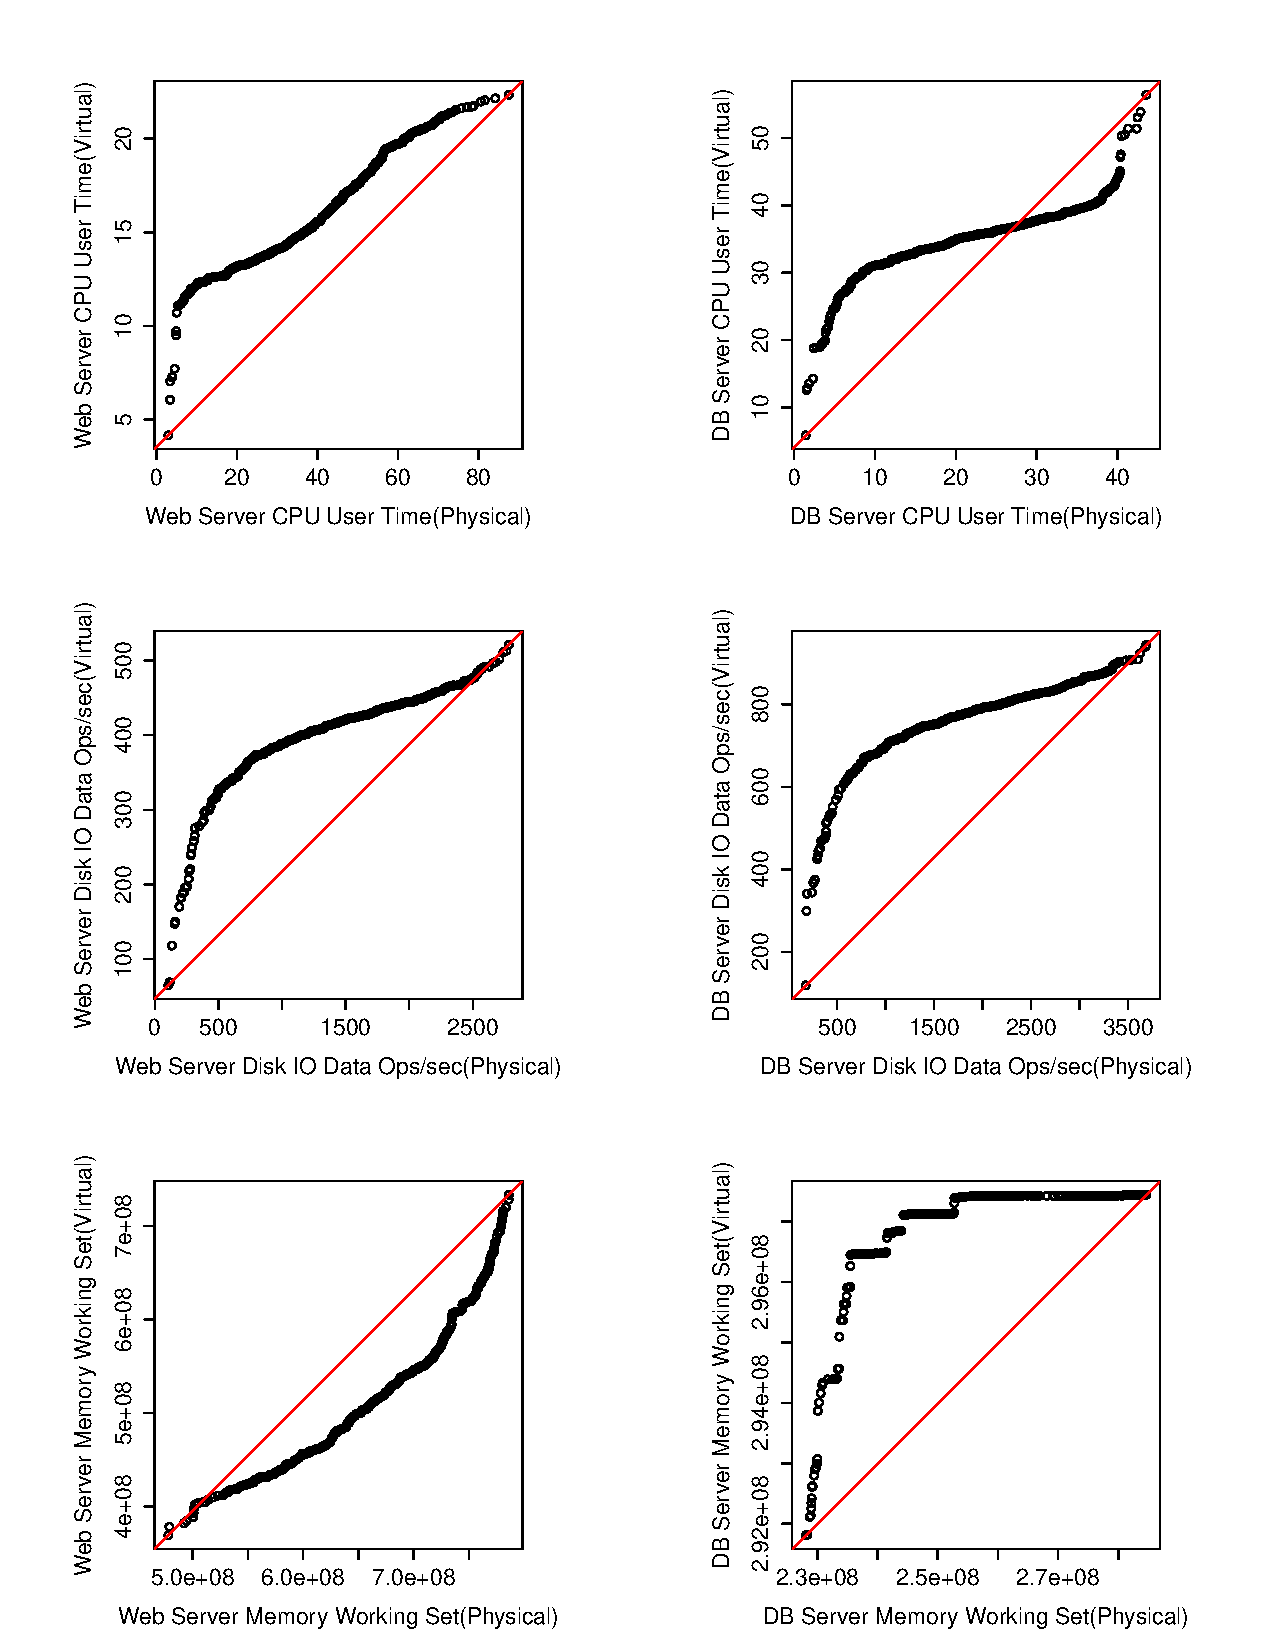
\includegraphics[width=0.9\columnwidth]{figures/CS_qq.pdf}
	\caption{Q-Q plots for CloudStore.}
	\label{fig:qqcs}
\end{figure}



%\footnote{The complete results, data and scripts are shared online at http://das.encs.concordia.ca/members/moiz-arif/}. 
The results show that the lines on the Q-Q plot are not close to the 45-degree reference line. By looking closely on the Q-Q plots we find that the patterns of each performance metric from different subject systems are different. For example, the application (web) server's CPU user time for DS2 in the virtual environment shows higher values than in the physical environment at the median to high range of the distribution; while the Q-Q plot of CloudStore shows the application (web) server's CPU user time with higher values at the low range of the distribution. In addition, the lines of the Q-Q plots for database memory working set show completely different shapes in DS2 and in CloudStore. The results imply that the discrepancies between virtual and physical environments are present between the subject systems. The impact of the subject systems warrants its own study.

The majority of the performance metrics had statistically significantly different distributions (p-values lower than 0.05 in Kolmogorov-Smirnov tests). Only 13 and 12 metrics (out of 44 for each environment) have p-values higher than 0.05, for DS2 and CloudStore, respectively, showing statistically in-significant difference between the distribution in virtual and physical environments. By looking closely at such metrics, we find that these metrics either do not highly relate to the execution of the subject system (e.g., application server CPU privileged time in DS2), or highly relate to the workload. Since the workload between the two environments is similar, it is expected that the metrics related to the workload follow the same shape of the distribution. For example, the I/O operations are highly related with the workload. The metrics related to I/O operations may show statistically in-significant differences between the distributions in the virtual and physical environments (e.g., application server I/O write operations per second in DS2). %\emad{should we list the metrics}


\noindent \textbf{Most performance metrics do not have the same trend in virtual and physical environments.} Table~\ref{tab:correlationrq1} shows the Spearman's rank correlation coefficient and corresponding p-value between the selected performance metrics for which we shared the Q-Q plots. We find that for the application server memory working set in CloudStore and the database server memory working set in DS2, there exists strong (0.69) to moderate (0.46) correlation between the virtual and physical environments, respectively. By examining the metrics, we find that both metrics have an increasing trend that may be caused by a memory leak. Such increasing trend may be the cause of the moderate to strong correlation. Instead of showing the selected metrics as the Q-Q plots, Table~\ref{tab:correlationall} shows a summary of the Spearman's rank correlation of all the performance metrics. Most of the correlations have an absolute value of 0 to 0.3 (low correlation), or the correlation is not statistically significant (p-val\textgreater0.05).

\noindent \textbf{Impact on the interpretation of examining single performance metric.} Practitioners often plot the trend of each important performance metrics, identify when the outliers exist or calculate the median or mean value of the metric to understand the performance of the system in general. However, based on our findings in this RQ, such analysis results may not be useful if they are from a virtual environment. For example, shown in Figures~\ref{fig:qqds2} and~\ref{fig:qqcs} many differences between the two distribution are in the lower and higher ends of the plots, which correspond to the high and low values of the metrics. Such values are often treated as outliers. However, if such outliers are due to the virtual environment rather than the system itself, the results may be misleading. In addition, since the distribution of the metrics are statistically different, the mean and median value of the metrics may also be misleading. 

\noindent\fbox{%
	\parbox{\textwidth}{%
		\textbf{Findings: }Performance metrics typically do not follow the same distribution in virtual and physical environments.\\ 
		\textbf{Actionable implications: }Practitioners cannot assume a straightforward overhead from the virtual environment nor compare single performance metric after applying a simple scaling factor to the metric.  
	}%
}




\begin{table}[thb]
	\centering
	\caption{Spearman's rank correlation coefficients and p-values of the highlighted performance metrics.}
	\label{tab:correlationrq1}
	\begin{tabular}{|c||c|c|c|c|}
		\hline
		\multirow{2}{*}{\textbf{Performance Metrics}} & \multicolumn{2}{c|}{\textbf{DS2}} & \multicolumn{2}{c|}{\textbf{CloudStore}} \\ \cline{2-5} 
		& \textbf{coef.} & \textbf{p-value} & \textbf{coef.} & \textbf{p-value} \\ %\hline
		\midrule 
		\midrule 
		Web Servers' User Times & 0.08 & 0.07 & -0.04 & 0.33 \\ \hline
		DB Servers User Times & -0.05 & 0.30 & 0.10 & 0.02 \\ \hline
		Web Servers' IO Data Ops/sec & 0.25 & 0.00 & 0.13 & 0.00 \\ \hline
		DB Servers' IO Data Ops/sec & -0.14 & 0.00 & 0.13 & 0.00 \\ \hline
		Web Servers' Memory Working Set & 0.22 & 0.00 & 0.69 & 0.00 \\ \hline
		DB Servers' Memory Working Set & 0.46 & 0.00 & -0.16 & 0.00 \\ \hline
	\end{tabular}
\end{table}

\begin{table}[tbh]
	\centering
	\caption{Summary of Spearman's rank correlation p-values and absolute coefficients of all the performance metrics in DS2 and CloudStore. The numbers in the table are the number of metrics that fall into each category.}
	\label{tab:correlationall}
	\begin{threeparttable}
		
		\begin{tabular}{|c||c|c|c|c|c|}
			\hline
			\multirow{3}{*}{\textbf{System}} & \multirow{3}{*}{\textbf{p-value\textgreater0.05}} & \multicolumn{4}{c|}{\textbf{p-value\textless0.05}} \\ \cline{3-6} 
			&  & \textbf{0.0$\sim$0.3} & \textbf{0.3$\sim$0.5} & \textbf{0.5$\sim$0.7} & \textbf{0.7$\sim$1} \\ %\hline
			\midrule 
			\midrule 
			\textbf{DS2} & 8 & 28 & 4 & 0 & 1 \\ \hline
			\textbf{CloudStore} & 5 & 25 & 4 & 4 & 3 \\ \hline
		\end{tabular}%
		\begin{tablenotes}
			\item Three metrics are constant. Therefore, we do not calculate the correlation on those metrics.
		\end{tablenotes}
	\end{threeparttable}
	
\end{table}



\subsection{To what extent does the relationship between the performance metrics change across environments?}

\label{sec:relation}

\noindent \textbf{Motivation.}
The relationship between two performance metrics may significantly change between two environments, which may be a hint of performance issues or system regression. 
%We have used the following approach to examine the relationships between the performance metrics. 
As found by Cohen \emph{et al$.$}~\cite{cohen2004correlating}, combinations of performance metrics are significantly more predictive towards performance issues than a single metric. A change in these combinations can reflect the discrepancy of performance and can help a practitioner identify the behavioral changes of a system between the two environments. For instance, in one release of the system, the CPU may be highly correlated with I/O while (e.g., when I/O is high, CPU is also high); while on a new release of the system, the correlation between CPU and I/O may become low. Such change to the correlation may expose a performance issue (e.g., the high CPU without I/O operation may be due to a performance bug). However, if there is a significant difference in correlations simply due to the platform being used, i.e., virtual vs. physical, then practitioners may need to be warned that a correlation discrepancy may be false. Therefore, we examine whether the relationship among performance metrics has a discrepancy between the virtual and physical environments. 
\\

\noindent \textbf{Approach.} 
We calculate Spearman's rank correlation coefficients among all the metrics from each performance test in each environment. Then we study whether such correlation coefficients are different between the virtual and physical environments. 

First, we compare the changes in correlation between the performance metrics and the system throughput. For example, in one environment, the system throughput may be highly correlated with CPU; while in another environment, such correlation is low. In such a case, we consider there to be a discrepancy in the correlation coefficient between CPU and the system throughput. Second, for every pair of metrics, we calculate the absolute difference between the correlation in two environments. For example, if CPU and Memory have a correlation of $0.3$ in the virtual environment and $0.5$ in the physical environment, we report the absolute difference in correlation as $0.2$ ($|0.3-0.5|$). Since we have 44 metrics in total, we plot a heatmap in order to visualize the 1,936 absolute difference values between every pair of performance metrics. The lighter the color for each block in the heatmap, the larger the absolute difference in correlation between a pair of performance metrics. With the heatmap, we can quickly spot the metrics that have large discrepancy in correlation coefficients. 
\\

\noindent \textbf{Results.}
\noindent \textbf{The correlations between system throughput and performance metrics change between virtual and physical environments.} Tables~\ref{tab:top10ds2p} and~\ref{tab:top10csp} present the top ten metrics with the highest correlations to system throughput in the physical environment for DS2 and CloudStore, respectively. We chose system throughput to be our criterion as it was kept identical between the environments.  We find that for these top ten metric sets, the difference in correlation coefficients in virtual and physical environments is up to \textbf{0.78} and the rank changes from \#9 to \#40 in DS2 and \#1 to \#10 in CloudStore.

\noindent \textbf{There exist differences in correlation among the performance metrics from virtual and physical environments.} Figures~\ref{fig:heatmap} and~\ref{fig:heatmap_cs} present the heatmap showing the changes in correlation coefficient among the performance metrics from virtual and physical environments. By looking at the heatmap, we find hotspots (with lighter color), which have larger correlation differences. For the sake of brevity, we do not show all the metric names in our heatmaps. Instead, we enlarge the heatmap by showing one of the hotspots for each subject system in Figures~\ref{fig:heatmap} and~\ref{fig:heatmap_cs}. We find that the hotspots correspond to the changes in correlation among I/O related metrics. Prior research on virtual machines has similar findings about I/O overhead in virtual machines~\cite{menon2005diagnosing,kraft2011io}. In such a situation, when practitioners observe that the relationship between I/O metrics and other metrics change, the change may not indicate a performance regression, but rather the change may be due to the use of a virtual environment.

\begin{figure}[tp]
	\centering
	{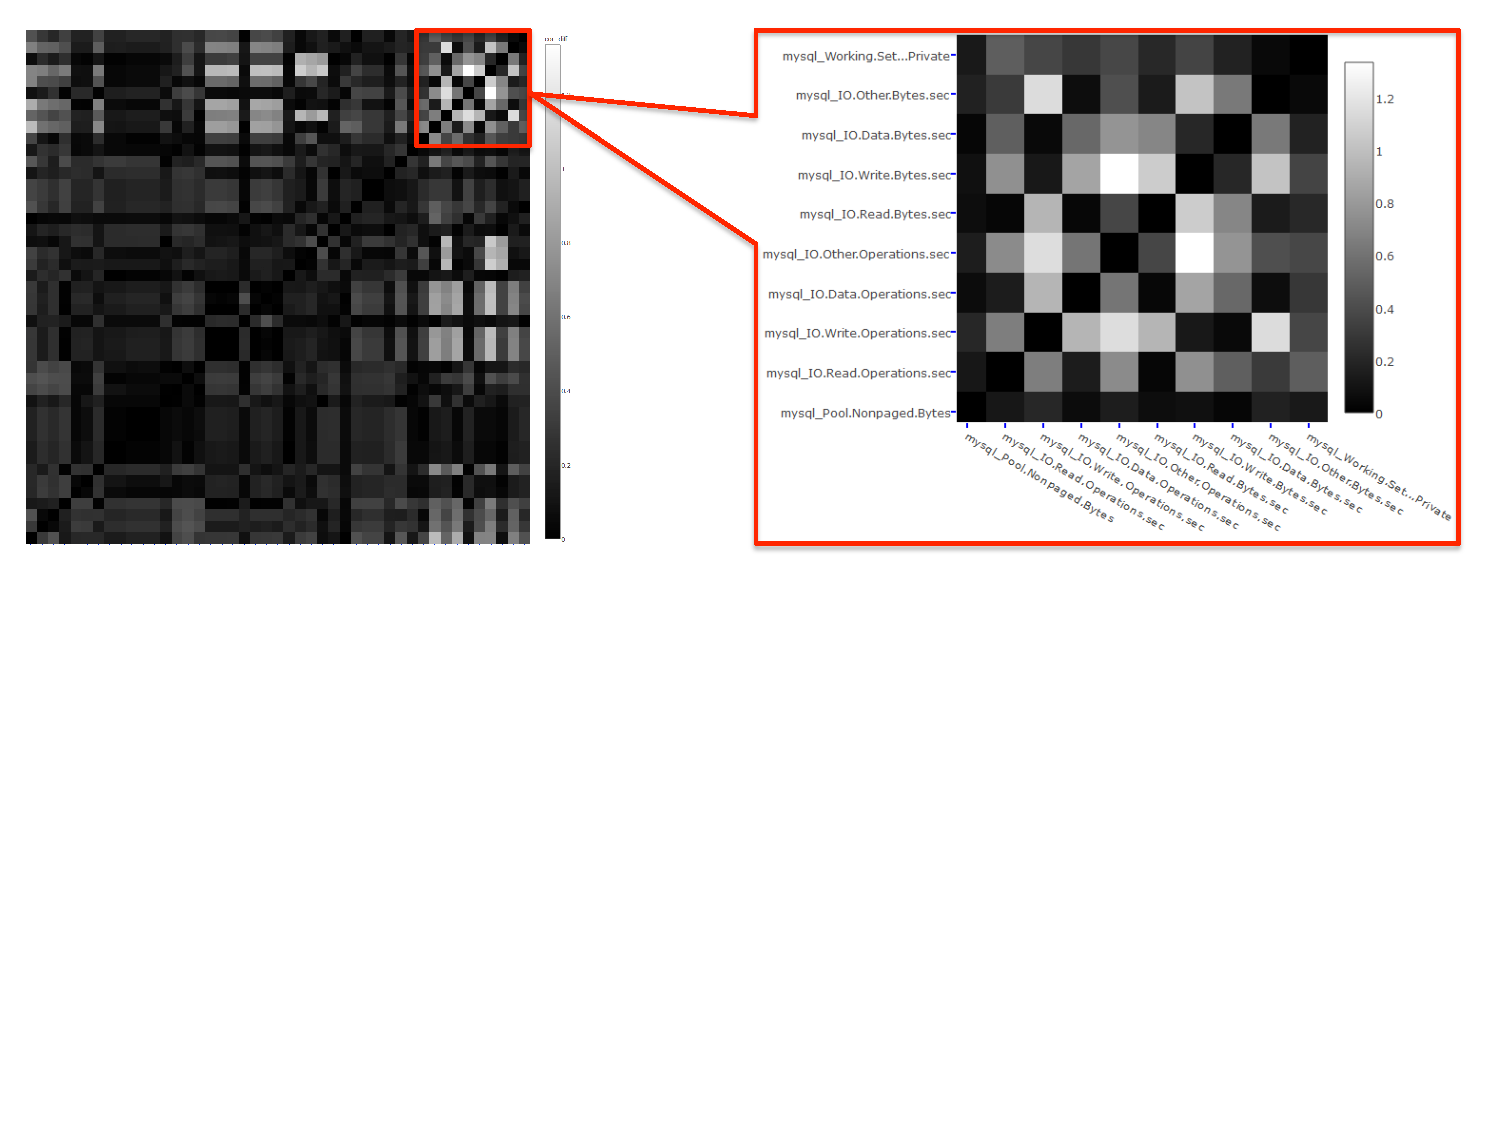
\includegraphics[width=1.0\textwidth]{figures/heatmap_DS2}}
	\caption{Heatmap of correlation changes for DS2.}
	%\captionsetup{justification=centering}
	\label{fig:heatmap}
\end{figure}


\begin{figure}[tp]
	\centering
	{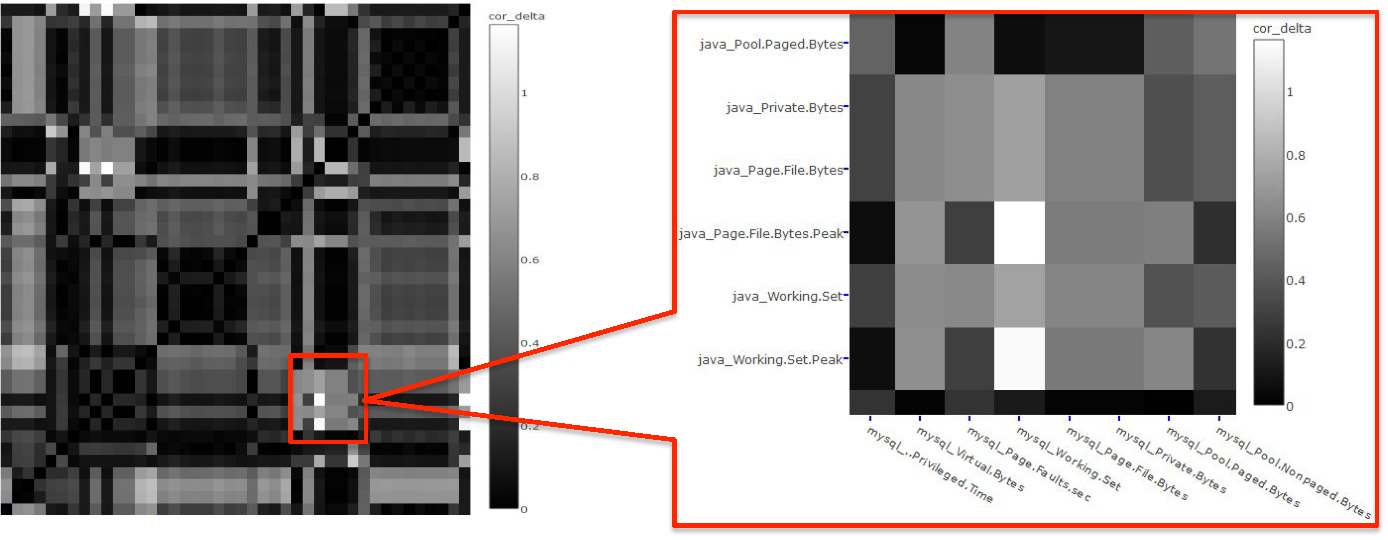
\includegraphics[width=1.0\textwidth]{figures/heatmap_CS}}
	\caption{Heatmap of correlation changes for CloudStore.}
	%\captionsetup{justification=centering}
	\label{fig:heatmap_cs}
\end{figure}




\noindent \textbf{Impact on the interpretation of examining correlations between performance metric.} When a system is reported to have performance issues, correlations between metrics are often used in practice, as describe in the motivation of this RQ. However, since such correlation can be inconsistent in virtual and physical environment, existing knowledge of assumptions of correlation may not exist or new correlation may emerge, due to the use of virtual environment. For example, practitioners of a database-centric system may have the knowledge that I/O traffic is correlated with CPU and system throughput. Examining these three metrics together can help diagnose performance issues, while if no such correlation exists in the virtual environment, these three metrics together may not be as useful in performance issue diagnosis.


\noindent\fbox{%
	\parbox{\textwidth}{%
		\textbf{Findings: }The correlations between performance metrics and system load may change considerably between virtual and physical environments. The correlation among performance metrics may also change considerably between virtual and physical environments. The correlations that are related with I/O metrics have the largest discrepancy.\\
		\textbf{Actionable implications: }Practitioners should always verify whether the inconsistency of correlations between performance metrics (especially I/O metrics) are due to virtual environments.
	}%
}






\begin{table}[tbh]
	\centering
	\caption{Top ten metrics with highest correlation coefficient to system throughput in the physical environment for DS2. }
	\label{tab:top10ds2p}
	\begin{threeparttable}
		
		\begin{tabular}{|c||c|c|c|c|}
			\hline
			\textbf{Rank} & \textbf{Performance } & \textbf{Coef. } & \textbf{Coef. } & \textbf{Rank in} \\ %\hline
			& \textbf{ Metrics} & \textbf{PE} & \textbf{VE} & \textbf{VE} \\ %\hline
			\midrule
			\midrule
			1 & Web IO Other Ops/sec & 0.91 & 0.62 & 10 \\ \hline
			2 & Web IO Other Bytes/sec & 0.91 & 0.62 & 12 \\ \hline
			3 & Web IO Write Ops/sec & 0.91 & 0.63 & 9 \\ \hline
			4 & Web IO Data Ops/sec & 0.91 & 0.63 & 8 \\ \hline
			5 & Web IO Write Bytes/sec & 0.90 & 0.62 & 11 \\ \hline
			6 & Web IO Data Bytes/sec & 0.90 & 0.61 & 13 \\ \hline
			7 & DB IO Other Ops/sec & 0.84 & 0.75 & 3 \\ \hline
			8 & DB IO Data Ops/sec & 0.83 & 0.07 & 41 \\ \hline
			9 & DB IO Other Bytes/sec & 0.83 & 0.15 & 40 \\ \hline
			10 & DB IO Read Ops/sec & 0.82 & 0.15 & 39 \\ \hline
		\end{tabular}%
		\begin{tablenotes}
			\item PE in the table is short for physical environment; while VE is short for virtual environment.
		\end{tablenotes}
	\end{threeparttable}
	
	
\end{table}

\begin{table}[tbh]
	\centering
	\caption{Top ten metrics with highest correlation coefficient to system throughput in the physical environment for CloudStore}
	\label{tab:top10csp}
	\begin{threeparttable}
		
		\begin{tabular}{|c||c|c|c|c|}
			\hline
			\textbf{Rank} & \textbf{Performance } & \textbf{Coef. } & \textbf{Coef. } & \textbf{Rank in} \\ %\hline
			& \textbf{ Metrics} & \textbf{PE} & \textbf{VE} & \textbf{VE} \\ %\hline
			\midrule
			\midrule
			1 & DB Server IO Other Bytes/sec & 0.98 & 0.73 & 10 \\ \hline
			2 & DB Server IO Read Ops/sec & 0.98 & 0.84 & 7 \\ \hline
			3 & DB Server IO Read Bytes/sec & 0.98 & 0.93 & 5 \\ \hline
			4 & DB Server IO Write Ops/sec & 0.98 & 0.97 & 2 \\ \hline
			5 & DB Server IO Data Ops/sec & 0.98 & 0.92 & 6 \\ \hline
			6 & DB Server IO Data Bytes/sec & 0.98 & 0.96 & 4 \\ \hline
			7 & DB Server IO Write Bytes/sec & 0.98 & 0.96 & 3 \\ \hline
			8 & Web Server IO Other Bytes/sec & 0.98 & 0.68 & 16 \\ \hline
			9 & DB Server IO Other Ops/sec & 0.98 & 0.98 & 1 \\ \hline
			10 & Web Server IO Other Ops/sec & 0.98 & 0.70 & 14 \\ \hline
		\end{tabular}%
		\begin{tablenotes}
			\item PE in the table is short for physical environment; while VE is short for virtual environment.
		\end{tablenotes}
	\end{threeparttable}
	
	
\end{table}


\subsection{Can statistical performance models be applied across virtual and physical environments?}
\label{sec:model}


\noindent \textbf{Motivation.}
As discussed in the last research question (see Section~\ref{sec:relation}), the relationship among performance metrics is critical for examining performance testing results (see Section~\ref{sec:relatedrelation}). However, thus far we have only examined the relationships between two performance metrics. In order to capture the relationship among a large number of performance metrics, more complex modeling techniques are needed. Hence, we use statistical modeling techniques to examine the relationship among a set of performance metrics~\cite{xiong2013vperfguard,cohen2004correlating}. Moreover, some performance metrics do not have any impact with system performance, which are still examined. For example, for a software system that is CPU intensive, I/O operations may be irrelevant. Such performance metrics may expose large discrepancies between virtual and physical environments while not contributing to the examination of performance testing results. It is necessary to remove such performance metrics that are not contributing or impacting the results of the performance analysis. To address the above issues, modeling techniques are proposed to examine performance testing results (see Section~\ref{sec:relatedmodel}). In this step, we examine whether the modeling among performance metrics can apply across virtual and physical environments and whether we can minimize such discrepancy between performance models.
\\

\noindent \textbf{Approach.}
We follow a model building approach that is similar to the approach from prior research~\cite{Shang:2015:ADP:2668930.2688052,Cohen:2005:CIC:1095810.1095821,xiong2013vperfguard}. We first build statistical models using performance metrics from one environment, then we test the accuracy of our performance model with the metric values from the same environment and also from a different environment. For example, if the model was built in a physical environment it was tested in both, physical and virtual environments.

\subsubsection{B-1: Reducing metrics}

Mathematically, performance metrics that show little or no variation do not contribute to the statistical models hence we first remove performance metrics that have constant values in the test results. We then perform a correlation analysis on the performance metrics to remove multicollinearity based on statistical analysis~\cite{cor_R}. We used the Spearman's rank correlation coefficient among all performance metrics from one environment. We find the pair of performance metrics that have a correlation higher than 0.75, as 0.75 is considered to be a high correlation~\cite{Syer2016}. From these two performance metrics, we remove the metric that has a higher average correlation with all other metrics. We repeat this step until there exists no correlation higher than 0.75.

We then perform redundancy analysis on the performance metrics. The redundancy analysis would consider a performance metric redundant if it can be predicted from a combination of other metrics~\cite{harrell2001regression}. We use each performance metric as a dependent variable and use the rest of the metrics as independent variables to build a regression model. We calculate the $R^2$ of each model. $R^2$, or the coefficient of multicollinearity, is used to analyze how a change in one of the variables (e.g. predictor) can be explained by the change in the second variable (e.g. response) \cite{rsquare}. We consider multicollinearity to be present if more than one predictor variable can explain the change in the response variable. If the $R^2$ is larger than a threshold (0.9)\cite{Syer2016}, the current dependent variable (i.e., performance metric) is considered redundant. We then remove the performance metric with the highest $R^2$ and repeat the process until no performance metric can be predicted with $R^2$ higher than the threshold. For example, if CPU can be linearly modeled by the rest of the performance metrics with $R^2\textgreater0.9$, we remove the metric for CPU.

Not all the metrics in the model are statistically significant. Therefore in this step, we only keep the metrics that have a statistically significant contribution to the model. We leverage the \textit{stepwise} function that adds the independent variables one by one to the model to exclude any metrics that are not contributing to the model~\cite{RInAction}. 

\subsubsection{B-2: Building statistical models}

In the second step, we build a linear regression model~\cite{freedman2009statistical} using the performance metrics that are left after the reduction and removal of statistically insignificant metrics in the previous step as independent variables and use the system throughput as our dependent variable. We chose the linear regression model over other models because of its simple explanation. Hence, it is easier to interpret the discrepancy that is illustrated by the model. Similar models have been built in prior research~\cite{Cohen:2005:CIC:1095810.1095821,xiong2013vperfguard,Shang:2015:ADP:2668930.2688052}.

%\subsubsection{B-3: Finalizing statistical models}
After removing all the insignificant metrics, we have all the metrics that significantly contribute to the model. We use these metrics as independent variables to build the final model.

\subsubsection{V-1: Validating model fit}

Before we validate the model with internal and external data, we first examine how good the model fit is. If the model has a poor fit to the data, then our findings from the model may be biased by the noise from the poor model quality. We calculate the $R^2$ of each model to measure fit. If the model perfectly fits the data, the $R^2$ of the model is 1, while a zero $R^2$ value indicates that the model does not explain the variability of the response data. We would also like to estimate the impact that each independent variable has on the model fit. We follow a ``drop one'' approach~\cite{Chambers1990}, which measures the impact of an independent variable on a model by measuring the difference in the performance of models built using: (1) all independent variables (the full model), and (2) all independent variables except for the one under test (the dropped model). A Wald statistic is reported by comparing the performance of these two models ~\cite{harrell2001regression}. A larger Wald statistic indicates that an independent variable has a larger impact on the model's performance, i.e., model fit. A similar approach has been leveraged by prior research in~\cite{mcintosh2015emse}. We then rank the independent variables by their impact on model fit. 


\subsubsection{V-2: Internal validation}

We validate our models with the performance testing data that is from the same environment. We leverage a standard 10-fold cross validation process, which starts by partitioning the performance data into 10 partitions. We take one partition (fold) at a time as the test set, and train on the remaining nine partitions~\cite{10foldcross,kohavi1995study}, similar to prior research~\cite{haroon}. For every data point in the testing data, we calculate the absolute percentage error. For example, for a data point with a throughput value of 100 requests per minute, if our predicted value is 110 requests per minute, the absolute percentage error is $0.1$ ($\frac{|110-100|}{100}$). After the ten-fold cross validation, we have a distribution of absolute percentage error (\textit{MAPE}) for all the data records.



\subsubsection{V-3: External validation}
To evaluate whether the model built using performance testing data in one environment (e.g., virtual environment) can apply to another environment (e.g., physical environment), we test the model using the data from the other environment.

Since the performance testing data is generated from different environments, directly applying the data on the model would intuitively generate large amounts of error. We adopt two approaches in order to normalize the data in different environments: (1) \textbf{Normalization by deviance.} The first approach we use is the same when we compare the distribution of each single performance metric shown in Equation~\ref{equ:mad} from Section~\ref{sec:individual} by calculating the relative deviance of a metric value from its median value. (2) \textbf{Normalization by load.} The second approach that we adopt is an approach that is proposed by Nguyen \textit{et al.}~\cite{Nguyen:2012:ADP:2188286.2188344}. The approach uses the load of the system to normalize the performance metric values across different environments. As there are varying inputs for the performance tests that we carried out, normalization by load helps in normalizing the multi-modal distribution that might be because of the trivial tasks like background processes(bookkeeping).



To normalize our metrics, we first build a linear regression model with the one metric as an independent variable and the throughput of the system as the dependent variable. With the linear regression model in one environment, the metric values can be represented by the system throughput. Then we normalize the metric value by the linear regression from the other environment. The details of the metric transformation are shown as follows:

\begin{equation*}
throughput_{p}= \alpha_{p} \times M_{p} + \beta_{p}
\end{equation*}
\vspace{-0.4cm}
\begin{equation*}
throughput_{v}= \alpha_{v} \times M_{v} + \beta_{v}
\end{equation*}
\vspace{-0.4cm}
\begin{equation*}
M_{normalized} = \frac{(\alpha_{v} \times M_{v})+\beta_{v}-\beta_{p}}{\alpha_{p}}
\end{equation*}
where $throughput_{p}$ and $throughput_{v}$ are the system throughput in the physical and virtual environment, respectively. $M_{p}$ and $M_{v}$ are the performance metrics from both environments, while $M_{normalized}$ is the metric after normalization. $\alpha$ and $\beta$ are the coefficient and intercept values for the linear regression models. After normalization, we calculate the absolute percentage error for every data record in the testing data.




\subsubsection{Identifying model discrepancy}
In order to identify the discrepancy between the models built using data from the virtual and physical environments, we compare the two distributions of absolute percentage error based on our internal and external validation. If the two distributions are significantly different (e.g., the absolute percentage error from internal validation is much lower than that from external validation), the two models are considered to have a discrepancy. To be more concrete, in total for each subject system, we ended up with four distributions of absolute percentage error: 1) modeling using the virtual environment and testing internally (on data from the virtual environment), 2) modeling using the virtual environment and testing externally (on data from the physical environment), 3) modeling using the physical environment and testing internally (on data from the physical environment), 4) modeling using the physical environment and testing externally (on data from the virtual environment). We compare distributions 1) and 2) and we compare distributions 3) and 4). Since normalization based on deviance will change the metrics values to be negative when the metric value is lower than median, such negative values cannot be used to calculate absolute percentage error. We perform a min-max normalization on the metric values before calculating the absolute percentage error. In addition, if the observed throughput value after normalization is zero (when the observed throughput value is the minimum value of both the observed and predicted throughput values), we cannot calculate the absolute percentage error for that particular data record. Therefore, we remove the data record if the throughput value after normalization is zero. In our case study, we only removed one data record when performing external validation with the model built in the physical environment. 
\\

\noindent \textbf{Results.}
\noindent \textbf{The statistically significant performance metrics leveraged by the models in virtual and physical environments are different.} Tables~\ref{tab:modelsummaryds2} and \ref{tab:modelsummarycs} show the summary of the statistical models built for the virtual and physical environments for the two subject systems. We find that all the models have a good fit (66.9\% to 94.6\% $R^2$ values). However, some statistically significant independent variables in one model do not appear in the other model. For example, Web Server Virtual Bytes ranks \#4 for the model built from the physical environment data of CloudStore, while the metric is not significant in the model built from the virtual environment data. In fact, none of the significant variables in the model built from the virtual environment are related to the application server's memory (see Table~\ref{tab:modelsummarycs}). We do observe some performance metrics that are significant in both models even with the same ranking. For example, Web Server IO Other Bytes/sec is the \#1 significant metric for both models built from the virtual and physical environment data of DS2 (see Table~\ref{tab:modelsummaryds2}). 

\noindent \textbf{The prediction error illustrates discrepancies between models built in virtual and physical environments.} Although the statistically significant independent variables in the models built by the performance testing results in the virtual and physical environments are different, the model may have similar prediction results due to correlations between metrics. However, we find that the external prediction errors are higher than internal prediction errors for all four models from the virtual and physical environments for the two subject systems. In particular, Table~\ref{tab:errors} shows the prediction errors using normalization based on load is always higher than that of the internal validation. For example, the median absolute percentage error for CloudStore using normalization by load is 632\% and 483\% for the models built in the physical environment and virtual environment, respectively; while the median absolute percentage error in internal validation is only 2\% and 10\% for the models built in the physical and virtual environments, respectively. However, in some cases, the normalization by deviance can produce low absolute percentage error in external validation. For example, the median absolute percentage error for CloudStore can be reduced to 9\% using normalization by deviance.\\ 
\indent One possible reason is that the normalization based on load performs better, even though it is shown to be effective in prior research~\cite{Nguyen:2012:ADP:2188286.2188344}, assumes a linear relationship between the performance metric and the system load. However, such an assumption may not be true in some performance testing results. For example, Table~\ref{tab:top10ds2p} shows that some I/O related metrics do have low correlation with the system load in virtual environments. On the other hand, the normalization based on deviance shows much lower prediction error. We think the reason is that the virtual environments may introduce metric values with high variance. Normalizing based on the deviance controls such variance, leading to lower prediction errors.



\begin{table}[tbh]
	\centering
	\caption{Summary of statistical models built for DS2. The metrics listed in the table are the significant independent variables.}
	\label{tab:modelsummaryds2}
	\resizebox{\columnwidth}{!}{%
		\begin{tabular}{|c||c|c|}
			\hline
			\textbf{Environment} & \textbf{Physical} & \textbf{Virtual} \\ %\hline
			\midrule
			\midrule
			\textbf{1} & Web Server IO Other Bytes/sec & Web Server IO Other Bytes/sec \\ \hline 
			\textbf{2} & Web Server Page Faults/sec & DB server Working Set - Peak \\ \hline
			\textbf{3} & DB Server Page Faults/sec & Web Server Virtual Bytes \\  \hline
			\textbf{4} & DB Server IO Write Bytes/sec & Web Server Page Faults/sec \\ \hline
			\textbf{5} & Web Server IO Read Bytes/sec & DB Server Page Faults/sec \\ \hline
			\textbf{6} & DB Server User Time & DB Server IO Data Ops/sec \\ \hline
			\textbf{7} & DB Server Pool Paged Bytes & -  \\ \hline
			\textbf{8} & DB Server Privileged Time &  - \\ \hline
			\midrule
			\textbf{$R^2$}  & 94.6\% & 66.90\% \\ \hline
			%			\textbf{MAPE} & 4.00\% & 10.52\% \\ \hline
		\end{tabular}%
	}
\end{table}


\begin{table}[tbh]
	\centering
	\caption{Summary of statistical models built for CloudStore. The metrics listed in the table are the significant independent variables.}
	\label{tab:modelsummarycs}
	\resizebox{\columnwidth}{!}{%
		\begin{tabular}{|c||c|c|}
			\hline
			\textbf{Environment} & \textbf{Physical} & \textbf{Virtual} \\ %\hline
			\midrule
			\midrule
			\textbf{1} & Web Server Privileged Time & Web Server IO Write Ops/sec \\ \hline
			\textbf{2} & DB Server Privileged Time & DB Server IO Read Ops/sec \\ \hline
			\textbf{3} & Web Server Page Faults/sec &  Web Server Privileged Time \\ \hline
			\textbf{4} & Web Server Virtual Bytes & DB Server Privileged Time \\ \hline
			\textbf{5} & Web Server Page File Bytes Peak &  DB Server IO Other Bytes/sec \\ \hline
			\textbf{6} & DB Server Pool Nonpaged Bytes & DB Server Pool Nonpaged Bytes \\ \hline
			\textbf{7} & DB Server Page Faults/sec & -  \\ \hline
			\textbf{8} & DB Server Working Set & - \\ %\hline
			\midrule
			\textbf{$R^2$} & 85.30\% & 90.20\% \\ \hline
			%		\textbf{MAPE} & 15.63\% & 3.65\% \\ \hline
		\end{tabular}%
	}
\end{table}
\begin{table}[tbh]
	\centering
	\caption{Internal and external prediction errors for both subject systems.}
	\label{tab:errors}
	\resizebox{\textwidth}{!}{%
		\begin{tabular}{|c||c|c|c|c|c|c|c|c|c|}
			\hline
			\multicolumn{9}{|c|}{\textbf{DS2}} \\ \hline
			\textbf{Model Built} & \multicolumn{2}{c|}{\textbf{Validation}} & \textbf{Min.} & \textbf{1st Quart.} & \textbf{Median} & \textbf{Mean} & \textbf{3rd Quart.} & \textbf{Max}\\ %\hline
			\midrule
			\midrule
			\multirow{3}{*}{\textbf{Physical}} & \multicolumn{2}{c|}{\textbf{Internal Validation}} & 0.00 & 0.01 & 0.02 & 0.03 & 0.05 & 0.30 \\ \cline{2-9} 
			& \multirow{2}{*}{\textbf{External Validation}} & \textbf{Normalization by Deviance} & 0.00 & 0.08 & 0.25 & 0.36 & 0.49 & 13.65 \\ \cline{3-9} 
			&  & \textbf{Normalization by Load} & 0.00 & 0.34 & 0.44 & 0.48 & 0.56 & 1.56  \\ \hline
			\multirow{3}{*}{\textbf{Virtual}} & \multicolumn{2}{c|}{\textbf{Internal Validation}} & 0.00 & 0.04 & 0.09 & 0.11 & 0.15 & 0.54 \\ \cline{2-9} 
			& \multirow{2}{*}{\textbf{External Validation}} & \textbf{Normalization by Deviance} & 0.00 & 0.09 & 0.20 & 0.27 & 0.34 & 2.82  \\ \cline{3-9} 
			&  & \textbf{Normalization by Load} & 0.00 & 0.06 & 0.13 & 0.17 & 0.23 & 0.92 \\ \hline
		\end{tabular}%
	}
	
	
	\vspace{2ex}
	
	\centering
	\resizebox{\textwidth}{!}{%
		\begin{tabular}{|c||c|c|c|c|c|c|c|c|}
			\hline
			\multicolumn{9}{|c|}{\textbf{CloudStore}} \\ \hline
			\textbf{Model Built} & \multicolumn{2}{c|}{\textbf{Validation}} & \textbf{Min.} & \textbf{1st Quart.} & \textbf{Median} & \textbf{Mean} & \textbf{3rd Quart.} & \textbf{Max}\\ \midrule
			\midrule
			\multirow{3}{*}{\textbf{Physical}} & \multicolumn{2}{c|}{\textbf{Internal Validation}} & 0.00 & 0..05 & 0.10 & 0.16 & 0.18 & 2.68\\ \cline{2-9} 
			& \multirow{2}{*}{\textbf{External Validation}} & \textbf{Normalization by Deviance} & 0.00 & 0.04 & 0.09 & 0.17 & 0.17 & 2.29  \\ \cline{3-9} 
			&  & \textbf{Normalization by Load} & 2.90 & 5.14 & 6.32 & 7.75 & 8.08 & 51.33 \\ \hline
			\multirow{3}{*}{\textbf{Virtual}} & \multicolumn{2}{c|}{\textbf{Internal Validation}} & 0.00 & 0.01 & 0.03 & 0.04 & 0.05 & 0.50  \\ \cline{2-9} 
			& \multirow{2}{*}{\textbf{External Validation}} & \textbf{Normalization by Deviance} & 0.00 & 0.03 & 0.07 & 0.11 & 0.13 & 1.00  \\ \cline{3-9} 
			&  & \textbf{Normalization by Load} & 4.07 & 4.64 & 4.83 & 5.13 & 5.10 & 33.36  \\ \hline
		\end{tabular}%
	}
	\vspace{-0.3cm}
\end{table}

\noindent \textbf{Impact on the interpretation of examining statistical performance models.} Statistical performance models are often used to interpret relationships among many system performance metrics. For example, what are the significant metrics that are associated with system load and what performance metrics are redundant. Since the statistical performance models have large discrepancy, even after applying normalization techniques that is proposed by prior research, we cannot directly use the performance models built in the virtual environment. Even though our results show that normalizing by deviance can reduce the discrepancy, practitioners should still be aware of it when examining the performance models.

\noindent\fbox{%
	\parbox{\textwidth}{%
		\textbf{Findings: }We find that the statistical models built by performance testing results in an environment cannot advocate for the other environment due to discrepancies present. Normalization technique for heterogeneous environments and workloads that is proposed by prior research may not work for virtual and physical environment.\\
		\textbf{Actionable implications: }Normalizing the performance metrics by deviance may minimize such discrepancy and should be considered by practitioners before examining performance testing results. 
	}%
}

In Chapter~\ref{chapter4}, we further validate our findings of Chapter~\ref{chapter3} by looking at external factors that may have affected the nature of our performance tests and the subsequent analysis.


\chapter{Summary, Contributions and Future Work}
\label{conclusion}
Performance assurance activities are vital in ensuring software reliability. Virtual environments are often used to conduct performance tests. However, the discrepancy between performance testing results in virtual and physical environments are never evaluated. In this paper, we evaluate such discrepancy by conducting performance tests on two open source systems (DS2 and CloudStore) in both virtual and physical environments. By examine the performance testing results, we find that there exist discrepancy between performance testing results in virtual and physical environments when examining individual performance metrics, relationship among performance metrics and building statistical models from performance metrics, even after we normalize performance metrics across different environments. The major contribution of this paper includes: 
\vspace{-0.15cm}
\begin{itemize} \itemsep -0.8pt 
	\item Our paper is the first research attempt to evaluate the discrepancy between performance testing results in virtual and physical environments.
	\item We find that relationships among I/O related metrics have large differences between virtual and physical environments.
	\item We find that normalizing performance metrics based on deviance may reduce the discrepancy. Practitioners may exploit such normalization techniques when analyzing performance testing results from virtual environments.
\end{itemize}
\vspace{-0.15cm}
Our results highlight the needs of awareness of discrepancy between performance testing results in virtual and physical environments, for both practitioners and researchers. Future research effort may focus on minimizing such discrepancy in order to improve the use of virtual environments in performance engineering and reliability assurance activities



%Our paper magnifies the impact of performance in difference environments. Additionally, we observed that the performance metrics from different environment do not belong to the same distribution. We tried to mitigate this impact by using scaled metrics in our performance regression models. As a result, the percentage error dropped drastically for one of our subject systems are increased for the other. We concluded that scaling may not apply to every subject system. We plan to see in what ways we can leverage the metrics from the virtual environment and use them for prediction of the metrics in the physical environment. We also plan to investigate the injection of regression in the system being hosted in a virtual environment will behave similar to that under regression in a physical environment. 

%\addcontentsline{toc}{chapter}{Bibliography}
\bibliography{bibliography.bib}  
\bibliographystyle{alpha}
\end{document}